\chapter{IIR滤波器的设计}
\begin{introduction}
    \item \textit{通过滤波器设计工具生成IIR滤波器系数;}
    \item \textit{使用MATLAB仿真IIR滤波器特性;}
    \item \textit{基于FPGA实现IIR滤波器并验证其功能;}
    \item \textit{分析设计的资源消耗与时序余量。}
    \item \textit{设计流程加速方法简述}
\end{introduction}

\section{实验背景与目的}
在数字信号处理领域,IIR滤波器的设计与实现同样具有重要意义。相较于FIR滤波器,IIR滤波器在满足同样滤波性能的情况下通常具有更低的阶数和更少的资源开销。使用FPGA厂商提供的IIR滤波器IP核可以简化设计流程,并提高设计的可靠性和实现效率。本实验旨在通过Xilinx IIR Filter IP核实现一个IIR滤波器,研究其实现过程,并分析其资源消耗与性能表现。

\section{实验原理}
\subsection{IIR Filter IP核简介}
Xilinx IIR Filter IP核是一个灵活且高效的IIR滤波器实现模块,支持多种滤波器类型(如巴特沃斯、切比雪夫等)和结构形式(如直接型II、级联型等)。该IP核允许用户根据具体应用需求,通过指定滤波器系数和控制参数来生成定制化的IIR滤波器。

\subsection{设计流程}
使用IIR Filter IP核设计IIR滤波器的基本流程如下:
\begin{enumerate}
    \item \textbf{确定滤波器参数:} 使用MATLAB或其他工具设计IIR滤波器并导出滤波器系数(如SOS矩阵); 
    \item \textbf{配置IP核:} 在Vivado中添加IIR Filter IP核,并根据设计需求配置其滤波器类型、结构形式、系数格式等参数;
    \item \textbf{生成IP核:} 生成配置好的IP核并将其集成至顶层设计中;
    \item \textbf{验证功能:} 通过仿真和上板测试,验证IIR滤波器在时域和频域上的表现,并评估其资源利用率和实时性能。
\end{enumerate}

\section{实验使用软件/平台}
\begin{itemize}
    \item Xilinx Vivado 2024.2;
    \item eNodeX 30B软件无线电创新平台;
    \item 示波器。
    \item MATLAB \& Simulink R2024b;
  \end{itemize}
\section{实验内容}
\subsection{滤波器系数生成}
使用MATLAB的\texttt{Filter Designer}工具生成IIR滤波器低通滤波器的系数,具体配置如下:
\begin{itemize}
    \item 滤波器类型:低通滤波器,Chebychev II型;
    \item 截止频率:12.5MHz;
    \item 采样频率:50MHz;
    \item 阶数:7;
    \item 节数(自动优化):4;
    \item 量化:12位定点数,最大精度。
\end{itemize}

图~\ref{fig:ex8:filter_coefficients}展示了生成的IIR滤波器的幅频和相频特性。可以看到,滤波器在800kHz以下的频率范围内具有良好的通带特性,而在12.5MHz以上的频率范围内则具有较好的阻带特性。量化前后幅频、相频特性均变化较小,不影响性能。相较FIR滤波器,其过渡带宽相对较宽。
\begin{figure}[htbp]
    \centering
    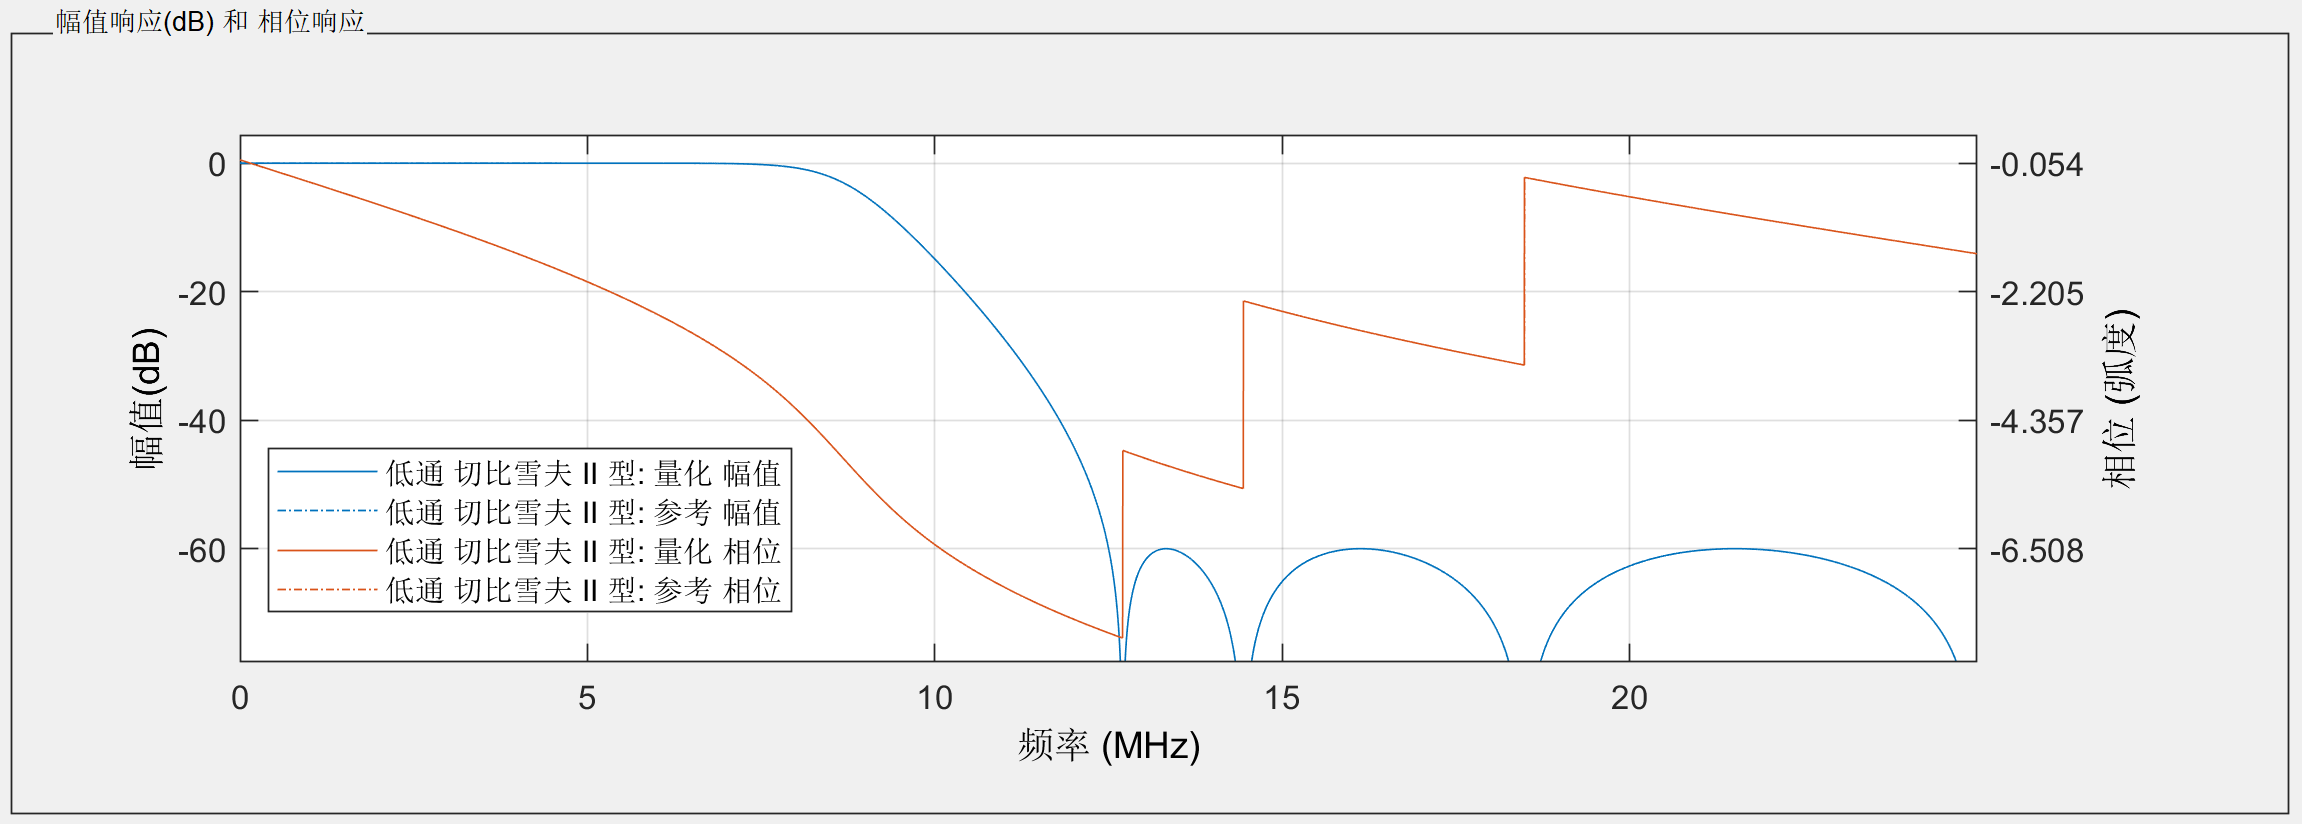
\includegraphics[width=0.8\textwidth]{figure/exp8/filterDesign.png}
    \caption{IIR滤波器参考/量化后幅频、相频特性}
    \label{fig:ex8:filter_coefficients}
\end{figure}

查看生成的滤波器系数,该滤波器系数将会在分子、分母计算的RTL代码中使用。


\subsection{IIR滤波器设计}
采用三个模块分别计算零点结果,极点结果和总结果。采用反馈结构进行计算,设计代码如下:
\begin{lstlisting}[language=verilog,caption={零点系数部分},label=lst:zp]
module ZeroParallel (
    input rst, // Reset signal, active high
    input clk, // FPGA system clock, 50MHz
    input signed [11:0] Xin, // Input data, 50MHz
    output signed [20:0] Xout // Output filtered data
);
 // Shift register for input samples
reg signed [11:0] Xin_Reg [6:0];
reg [3:0] i, j;
always @(posedge clk or posedge rst) begin
    if (rst) begin
        for (i = 0; i < 7; i = i + 1)
            Xin_Reg[i] <= 12'd0;
    end else begin
        for (j = 0; j < 6; j = j + 1)
            Xin_Reg[j+1] <= Xin_Reg[j];
        Xin_Reg[0] <= Xin;
    end
end
// Sum symmetric inputs
wire signed [12:0] Add_Reg [3:0];
assign Add_Reg[0] = Xin + Xin_Reg[6];
assign Add_Reg[1] = Xin_Reg[0] + Xin_Reg[5];
assign Add_Reg[2] = Xin_Reg[1] + Xin_Reg[4];
assign Add_Reg[3] = Xin_Reg[2] + Xin_Reg[3];
// Multiply by coefficients using shifts and additions
wire signed [20:0] Mult_Reg [3:0];
assign Mult_Reg[0] = {{6{Add_Reg[0][12]}}, Add_Reg[0], 2'd0}
+ {{7{Add_Reg[0][12]}}, Add_Reg[0], 1'd0}
+ {{8{Add_Reg[0][12]}}, Add_Reg[0]}; // *7
assign Mult_Reg[1] = {{4{Add_Reg[1][12]}}, Add_Reg[1], 4'd0}
+ {{6{Add_Reg[1][12]}}, Add_Reg[1], 2'd0}
+ {{8{Add_Reg[1][12]}}, Add_Reg[1]}; // *21
assign Mult_Reg[2] = {{3{Add_Reg[2][12]}}, Add_Reg[2], 5'd0}
+ {{5{Add_Reg[2][12]}}, Add_Reg[2], 3'd0}
+ {{7{Add_Reg[2][12]}}, Add_Reg[2], 1'd0}; // *42
assign Mult_Reg[3] = {{3{Add_Reg[3][12]}}, Add_Reg[3], 5'd0}
+ {{4{Add_Reg[3][12]}}, Add_Reg[3], 4'd0}
+ {{5{Add_Reg[3][12]}}, Add_Reg[3], 3'd0}; // *56
// Sum results
assign Xout = Mult_Reg[0] + Mult_Reg[1] + Mult_Reg[2] + Mult_Reg[3];
endmodule
\end{lstlisting}
\begin{lstlisting}[language=verilog,caption={极点系数部分}]
module PoleParallel (
    input rst, // Reset signal, active high
    input clk, // FPGA system clock, 50MHz
    input signed [11:0] Yin, // Input data, 50MHz
    output signed [25:0] Yout // Output filtered data
);
// Shift register for previous outputs
reg signed [11:0] Yin_Reg [6:0];
reg [3:0] i, j;
always @(posedge clk or posedge rst) begin
    if (rst) begin
        for (i = 0; i < 7; i = i + 1)
            Yin_Reg[i] <= 12'd0;
    end else begin
        for (j = 0; j < 6; j = j + 1)
            Yin_Reg[j+1] <= Yin_Reg[j];
        Yin_Reg[0] <= Yin;
    end
end

// Coefficients (12-bit signed)
wire signed [11:0] coe [7:0];
assign coe[1] = -12'd922;
assign coe[2] = 12'd1163;
assign coe[3] = -12'd811;
assign coe[4] = 12'd412;
assign coe[5] = -12'd122;
assign coe[6] = 12'd24;
assign coe[7] = -12'd2;

// Multiplier outputs
wire signed [22:0] Mult_Reg [6:0];
MULT Umult1 (.A(coe[1]), .B(Yin_Reg[0]), .P(Mult_Reg[0]));
MULT Umult2 (.A(coe[2]), .B(Yin_Reg[1]), .P(Mult_Reg[1]));
MULT Umult3 (.A(coe[3]), .B(Yin_Reg[2]), .P(Mult_Reg[2]));
MULT Umult4 (.A(coe[4]), .B(Yin_Reg[3]), .P(Mult_Reg[3]));
MULT Umult5 (.A(coe[5]), .B(Yin_Reg[4]), .P(Mult_Reg[4]));
MULT Umult6 (.A(coe[6]), .B(Yin_Reg[5]), .P(Mult_Reg[5]));
MULT Umult7 (.A(coe[7]), .B(Yin_Reg[6]), .P(Mult_Reg[6]));
// Sum multiplier outputs
assign Yout = Mult_Reg[0] + Mult_Reg[1] + Mult_Reg[2]
+ Mult_Reg[3] + Mult_Reg[4] + Mult_Reg[5] + Mult_Reg[6];
endmodule
\end{lstlisting}
\begin{lstlisting}[language=verilog,caption={IIR滤波器整合}]
module IIRDirect (
    input rst, // Reset signal, active high
    input clk, // FPGA system clock, 50MHz
    input signed [11:0] din, // Input data
    output signed [11:0] dout // Output filtered data
);
// Instantiate Zero Parallel block
wire signed [20:0] Xout;
ZeroParallel U0 (
    .rst(rst),
    .clk(clk),
    .Xin(din),
    .Xout(Xout)
);
// Instantiate Pole Parallel block
wire signed [11:0] Yin;
wire signed [25:0] Yout;
PoleParallel U1 (
    .rst(rst),
    .clk(clk),
    .Yin(Yin),
    .Yout(Yout)
);
// Calculate output: (Zero - Pole) / 512
wire signed [25:0] Ysum;
assign Ysum = {{5{Xout[20]}}, Xout} - Yout;
wire signed [25:0] Ydiv;
assign Ydiv = {{9{Ysum[25]}}, Ysum[25:9]}; // Arithmetic shift right by 9 (divide by
512)
// Final output assignment
assign Yin = (rst ? 12'd0 : Ydiv[11:0]);
assign dout = Yin;
endmodule
\end{lstlisting}
\subsection{仿真测试}
Testbench代码如代码~\ref{lst:iir_ip_tb}所示,使用Vivado的仿真工具进行功能验证。采用\textit{Clock Wizard}产生50MHz仿真时钟,输入激励分别为:
\begin{itemize}
    \item 两个不同频率的正弦波叠加信号;
    \item 白噪声信号。
\end{itemize}

输入激励信号由MATLAB生成(也可以使用自动生成框架中的\texttt{gen\_sine\_wave}函数,代码如下。
\begin{lstlisting}
    [language=matlab,caption={MATLAB生成激励代码},label=lst:fir_ip_tb_matlab]
    %sim_data_gen.m
    clc;
    clear 
    f1=1e6;       %信号1频率1MHz
    f2=10e6;     %信号2频率10MHz
    Fs=50e6;      %采样频率50MHz
    N=12;               %量化位数
    data_len = 2000; %生成数据长度
    
    %产生频率叠加信号
    t=0:1/Fs:(data_len-1)/Fs;
    c1=2*pi*f1*t;
    c2=2*pi*f2*t;
    s=sin(c1)+sin(c2);       
    
    %产生白噪声信号
    noise=randn(1,length(t));%产生高斯白噪声数据
    
    %归一化处理
    noise=noise/max(abs(noise));
    s=s/max(abs(s));
    
    %N位量化处理
    Q_noise=round(noise*(2^(N-1)-1));
    Q_s=round(s*(2^(N-1)-1));
    
    %绘制产生数据的时域图
    figure(1)
    subplot(211)
    plot(t(1:300),Q_s(1:300));
    xlabel('时间(s)');ylabel('幅度(v)');
    legend ('频率叠加信号');
    grid on;
    
    subplot(212)
    plot(t(1:200),Q_noise(1:200));
    xlabel('时间(s)');ylabel('幅度(v)');
    legend('白噪声信号');
    grid on;
    
    
    %求输入信号的频谱响应
    f_s=abs(fft(Q_s,1024));
    f_s=20*log10(f_s);
    f_noise=abs(fft(Q_noise));
    f_noise=20*log10(f_noise);
    
    f_s=f_s-max(f_s);
    f_noise=f_noise-max(f_noise);
    
    
    figure(2)
    subplot(211)
    L=length(f_s);
    %横坐标单位设置为MHz
    xf=0:L-1;
    xf=xf*Fs/L/10^6;     
    plot(xf(1:L/2),f_s(1:L/2));
    xlabel('频率(MHz)');ylabel('幅度(dB)');
    legend('频率叠加信号信号');
    grid on;
    
    subplot(212)
    plot(xf(1:L/2),f_noise(1:L/2));
    xlabel('频率(MHz)');ylabel('幅度(dB)');
    legend('白噪声信号');
    grid on;
    
    fid=fopen('./Bin_noise12.txt','w');
    for i=1:length(Q_noise)
        B_noise=dec2bin(Q_noise(i)+(Q_noise(i)<0)*2^N,N);
        for j=1:N
           if B_noise(j)=='1'
               tb=1;
           else
               tb=0;
           end
           fprintf(fid,'%d',tb);  
        end
        fprintf(fid,'\r\n');
    end
    fprintf(fid,';'); 
    fclose(fid);
    
    fid=fopen('./Bin_sin12.txt','w');
    for i=1:length(Q_s)
        B_s=dec2bin(Q_s(i)+(Q_s(i)<0)*2^N,N);
        for j=1:N
           if B_s(j)=='1'
               tb=1;
           else
               tb=0;
           end
           fprintf(fid,'%d',tb);  
        end
        fprintf(fid,'\r\n');
    end
    fprintf(fid,';'); 
    fclose(fid);
    \end{lstlisting}
输出为经过IIR滤波器处理后的信号。
\begin{lstlisting}[language=verilog,caption={IIR滤波器的Testbench},label=lst:iir_ip_tb]
`timescale 1ns / 1ps
module tb_IIR(
);
// Inputs
reg rst;
reg clk;
reg signed [11:0] Xin;
// Outputs
wire signed [11:0] Yout;
initial begin
    // Initialize Inputs
    rst = 1;
    clk = 0;
    // Wait 100 ns for global reset to finish
    #100;
    rst = 0;
    // Add stimulus here
end
always #10 clk <= !clk;
IIRDirect sim(
    .rst(rst),
    .clk(clk), //系统时钟 50MHz
    .din(Xin), //输入数据
    .dout(Yout) //输出数据
);
//从外部 i 文件读入数据作为测试激励
integer i = 0;
parameter sim_len = 2000;
reg [11:0] sim_data[1:sim_len];
always @(posedge clk) begin
//
    $readmemb("./Bin_sin12.txt",sim_data);
    // $readmemb("./Bin_noise12.txt",sim_data);
    i = i + 1;
    Xin=sim_data[i];
end
//将仿真数据 dout 写入外部 TXT 文件中
integer file_out;
initial begin
//
file_out = $fopen("./sin_filter_out.txt");
// file_out = $fopen("./noise_filter_out.txt");
if(!file_out) begin
    $display("could not open file!");
    $finish;
end
end
//将输出数据写入指定文本文件中
wire rst_write;
//产生写入时钟信号,复位状态时不写入数据
assign rst_write = clk & (!rst);
always @(posedge rst_write)
$fdisplay(file_out,"%d",Yout);
endmodule
\end{lstlisting}

波形仿真结果(图~\ref{fig:exp8:sim_result}~)表明,滤波器能够有效滤除白噪声中的高频分量,保留低频分量。

\begin{figure}[htbp]
    \centering
    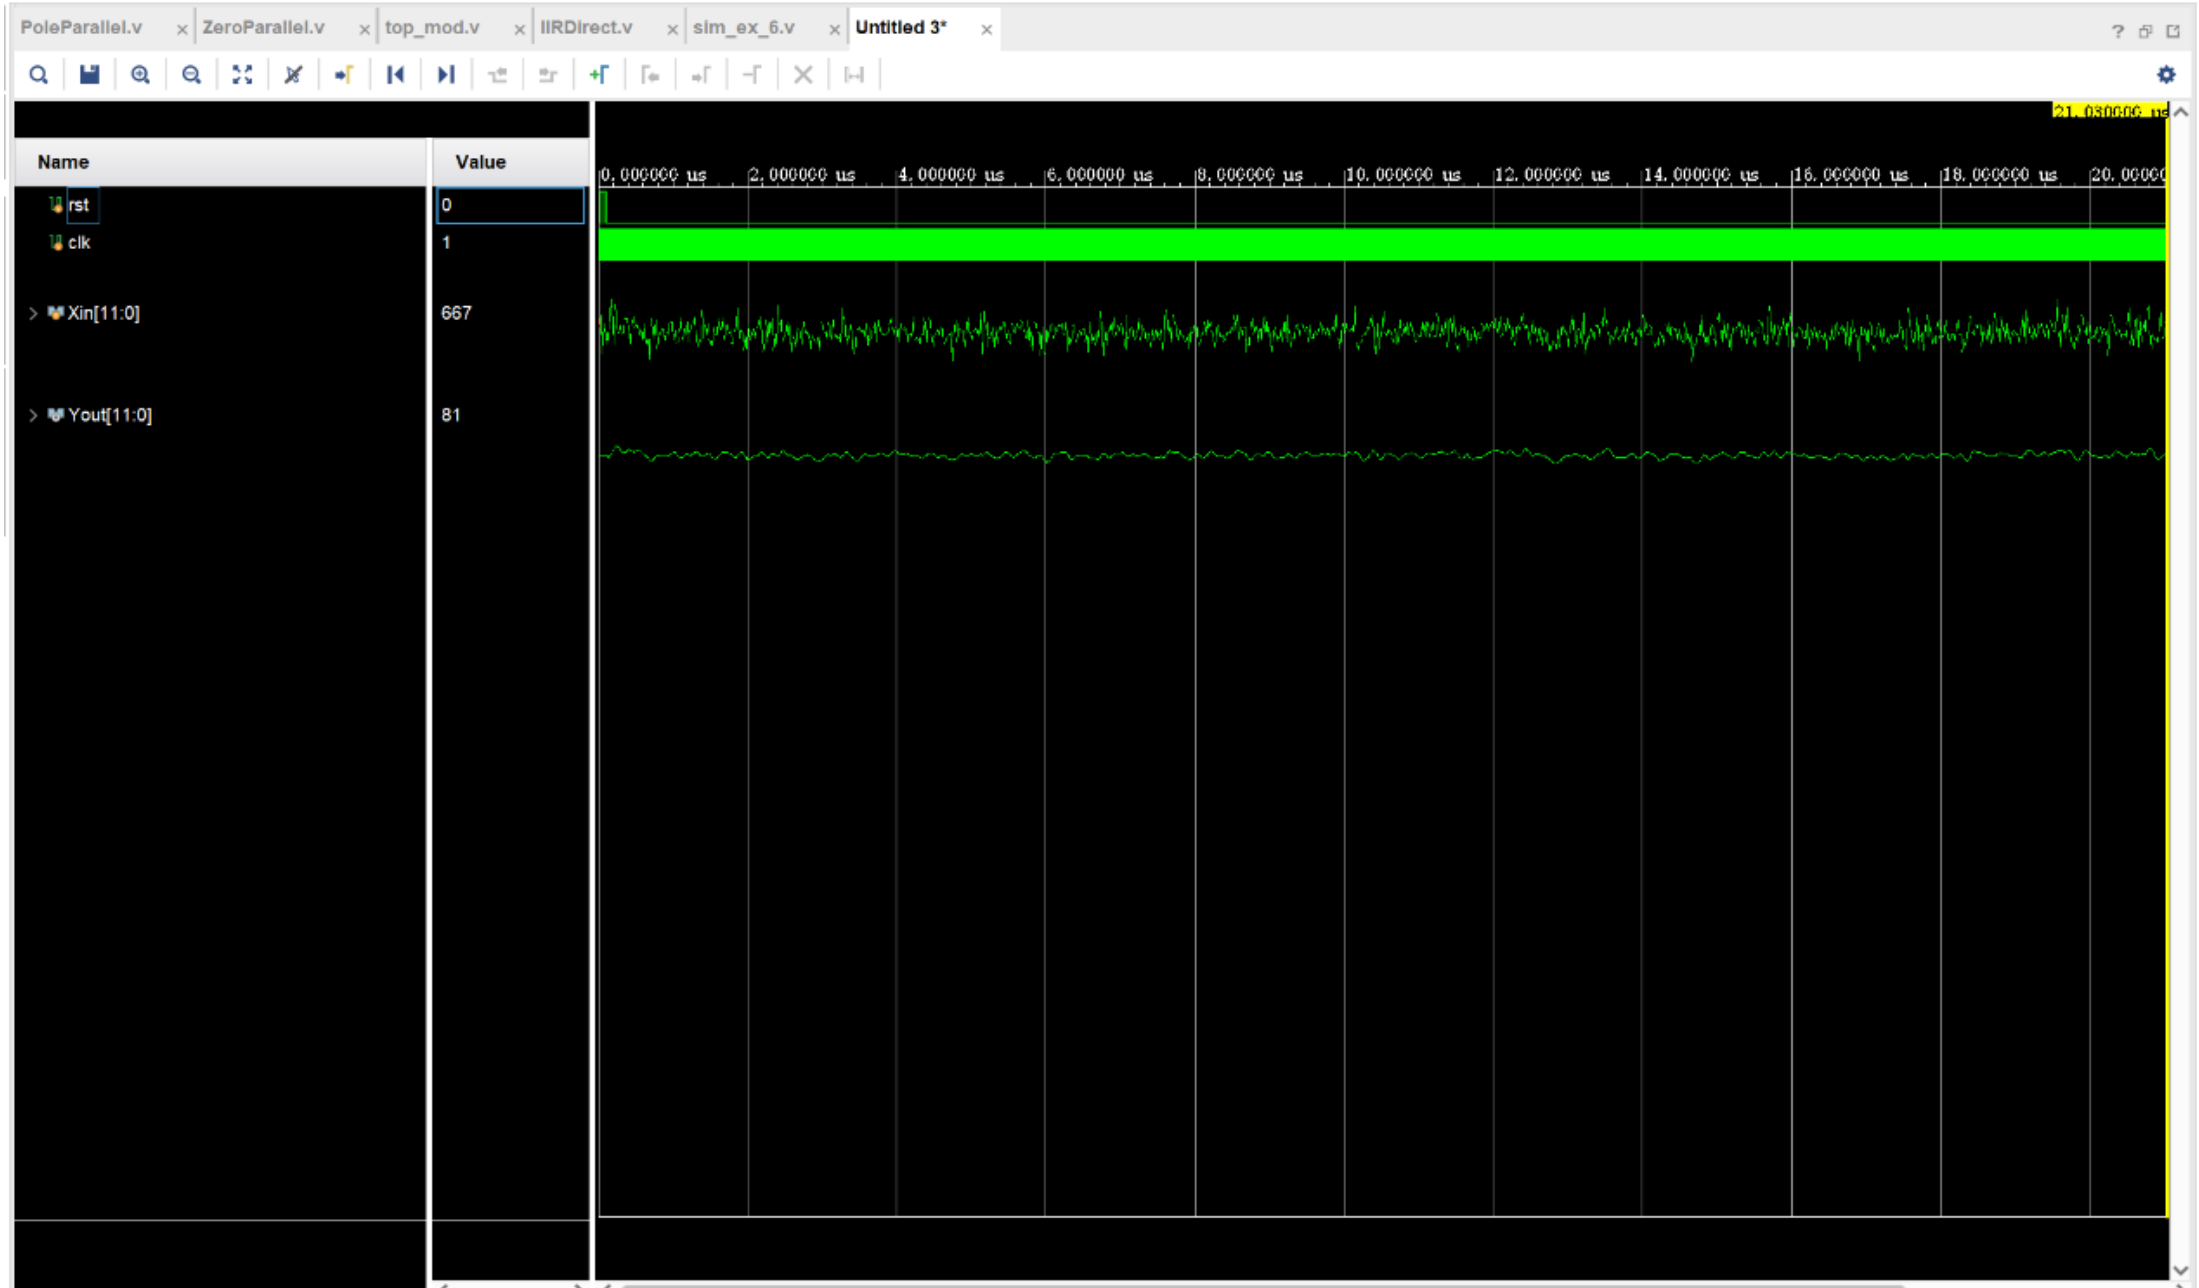
\includegraphics[width = 0.85\textwidth]{figure/exp8/sim_noise.png}
    \caption{仿真结果} 
    \label{fig:exp8:sim_result}   
\end{figure}

将仿真文件输出的结果写入文本文件中,使用MATLAB进行后续分析。MATLAB代码如下(代码~\ref{lst:fir_ip_tb_matlab}~),绘制了经过滤波器处理后的信号的幅频响应曲线。可以看到,经过滤波器处理后,信号的高频分量被有效滤除,保留了低频分量。
\begin{lstlisting}[language=matlab,caption={MATLAB结果绘图代码},label=lst:fir_ip_tb_matlab]
%sim_data_Analyse.m
%采样频率为50MHz
clear;
Fs=50e6;        
%从文本文件中读取数据
fid=fopen('./sin_filter_out.txt','r');
%fid=fopen('D:\dsp_lab_data\noise_filter_out.txt','r');
[dout,count]=fscanf(fid,'%lg',inf);
fclose(fid);

%求信号的幅频响应
f_out=20*log10(abs(fft(dout,1024)));
f_out=f_out-max(f_out);

%设置幅频响应的横坐标单位为MHz
x_f=[0:(Fs/length(f_out)):Fs/2]/10^6;
%只显示正频率部分的幅频响应
mf_noise=f_out(1:length(x_f));

%绘制幅频响应曲线
plot(x_f,mf_noise);
xlabel('频率(MHz)');ylabel('幅度(dB)');
grid on;

\end{lstlisting}

\begin{figure}[htbp]
    \centering
    \subfloat[频率叠加与白噪声信号输入时域波形]{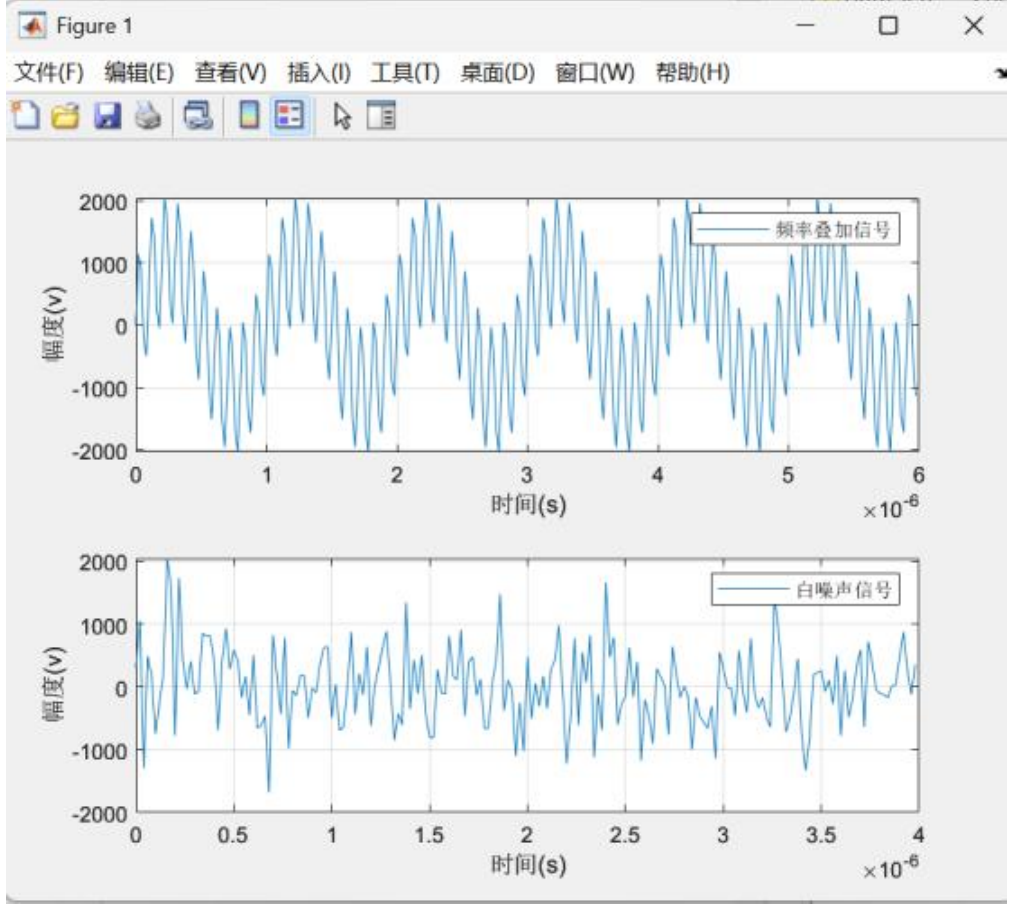
\includegraphics[width=0.45\textwidth]{figure/exp7/mat_1.png}}
    \hfill
    \subfloat[频率叠加与白噪声信号输入频谱]{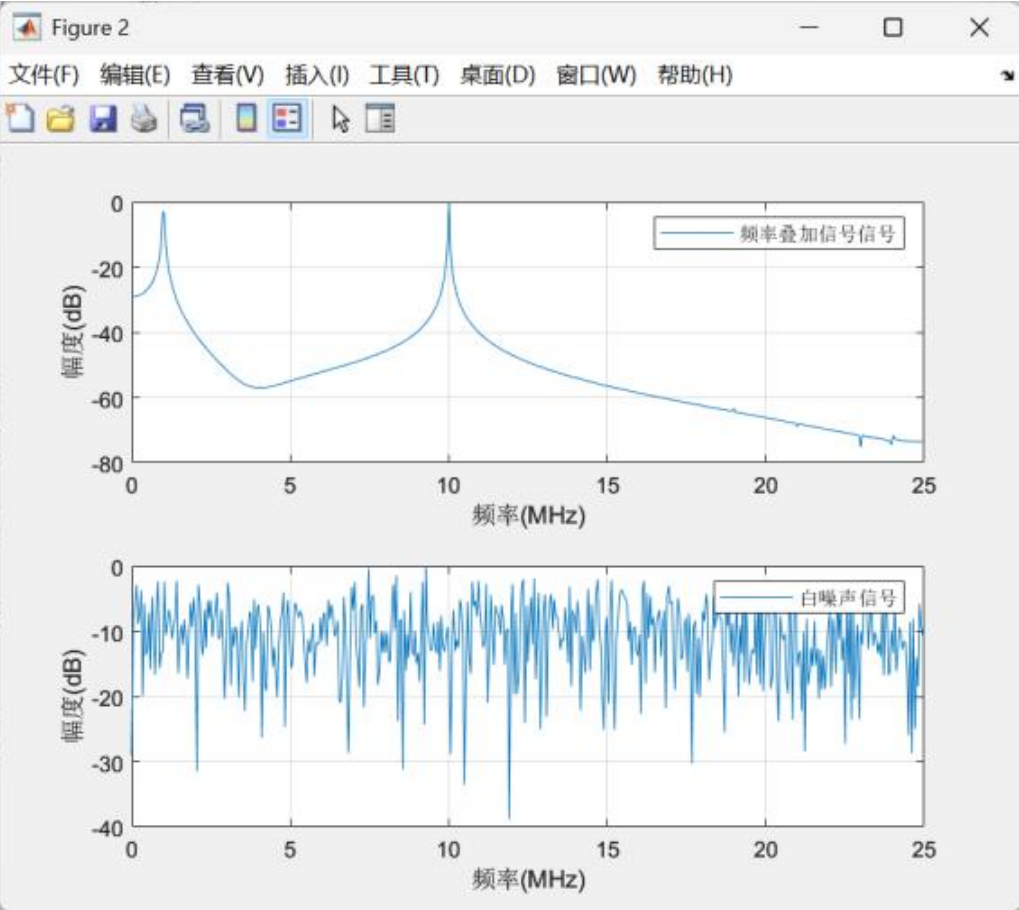
\includegraphics[width=0.45\textwidth]{figure/exp7/mat_2.png}}
    \\
    \subfloat[频率叠加信号滤波输出频谱]{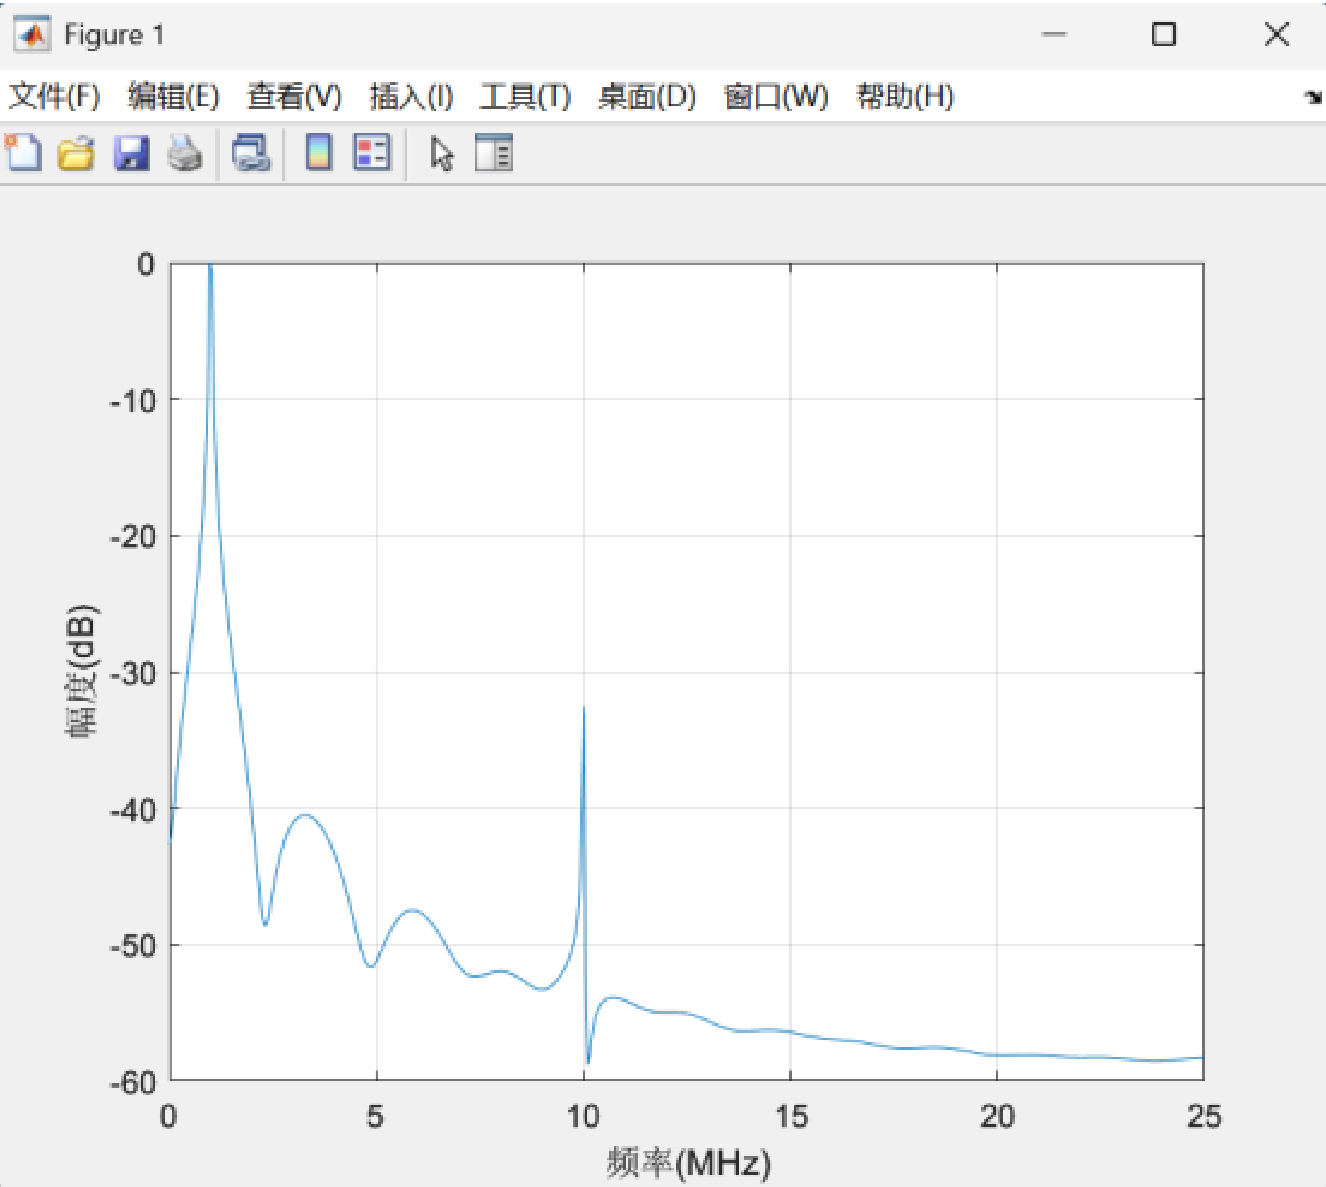
\includegraphics[width=0.45\textwidth]{figure/exp7/mat_3.png}}
    \hfill
    \subfloat[白噪声信号滤波输出频谱]{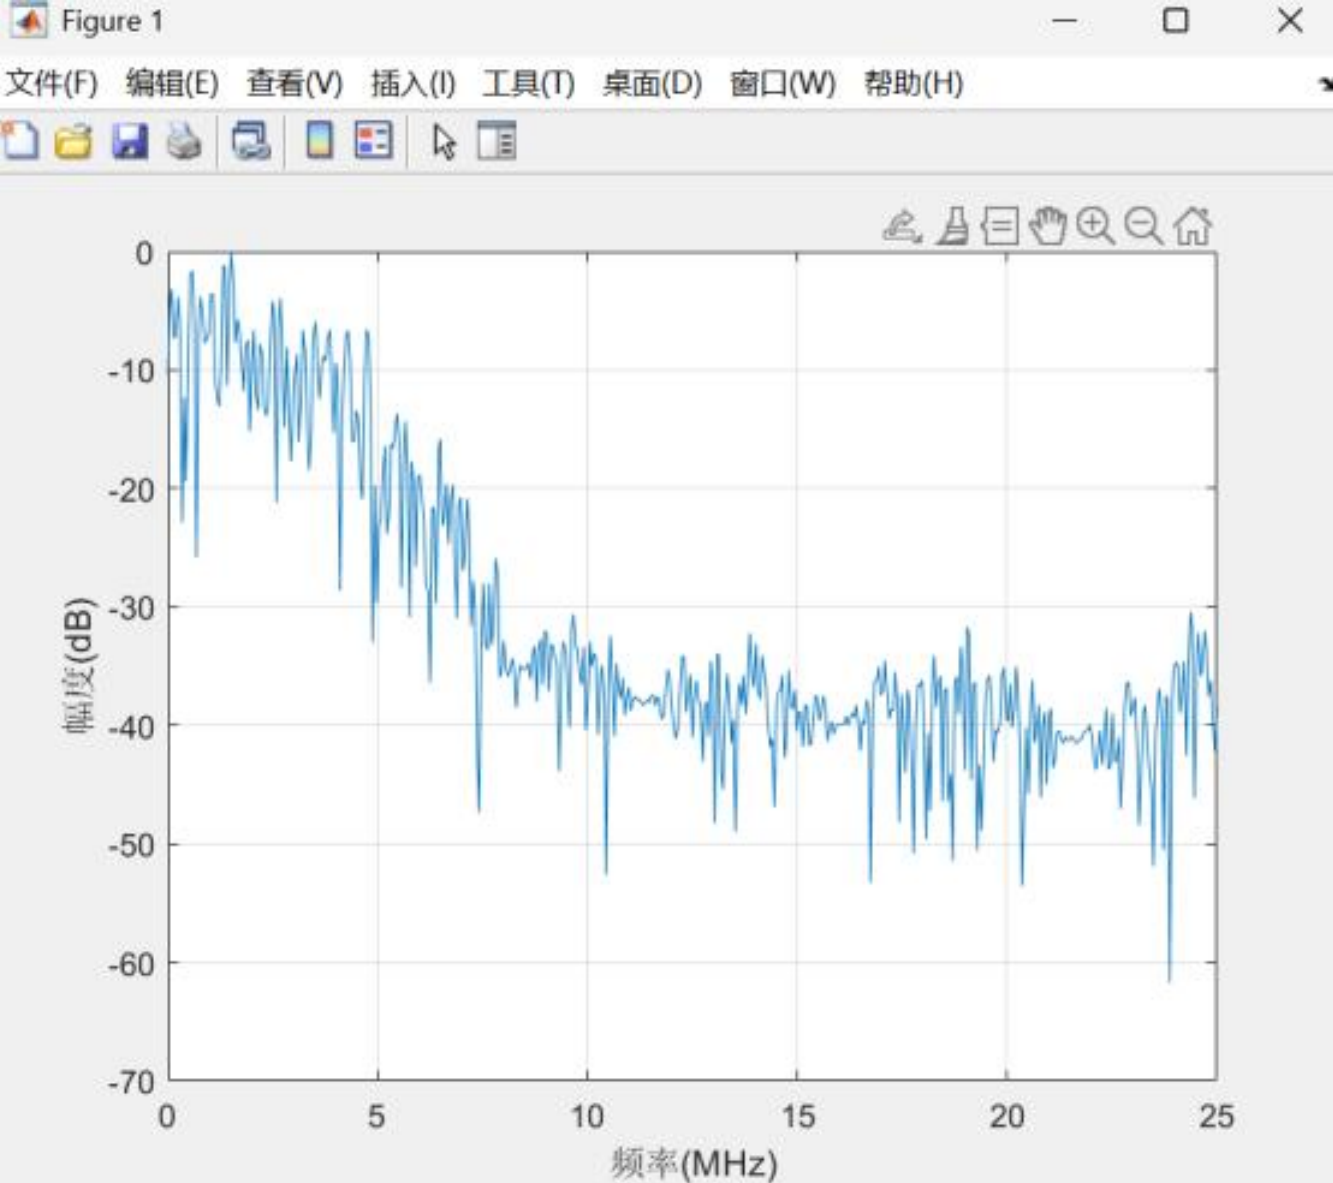
\includegraphics[width=0.45\textwidth]{figure/exp7/mat_4.png}}
    \caption{MATLAB分析的输入信号与滤波结果}
    \label{fig:exp7:matlab_results}
\end{figure}
\subsection{硬件实现与验证}
将生成的IIR滤波器集成到设计中,连接板载输入输出信号,并通过ILA波形和示波器波形验证滤波器的功能。测试输入信号为叠加的250kHz和4MHz正弦波,测试时钟为20MHz,验证滤波器是否能够有效滤除4MHz分量。

顶层模块代码如下:
\begin{lstlisting}[language=verilog,caption={顶层模块代码},label=lst:top_module]
`timescale 1ns / 1ps
module top_mod (
               // DAC PINS
               output signed [13:0] LS_DAC2_DB,
               output LS_DAC2_CLK,
               output LS_DAC2_WRT,
               output signed [13:0] LS_DAC1_DB,
               output LS_DAC1_CLK,
               output LS_DAC1_WRT,
    
               output LS_DAC_MODE,
    
    
               // ADC PINS
               input [11:0] LS_ADC2_DB,
               input [11:0] LS_ADC1_DB,
               input LS_ADC2_OTR,
               input LS_ADC1_OTR,
               output LS_ADC2_CLK,
               output LS_ADC1_CLK,
    
               // GPIOs IO PINs
               // output GPIO_TH1, GPIO_TH2, GPIO_TH3, GPIO_TH4, GPIO_TH5,
               // output GPIO_TH6, GPIO_TH7, GPIO_TH8, GPIO_TH9, GPIO_TH10
    
               input PL_CLK_100MHz  // Clk 100MHz
           );
    
    wire clk_20M;
    wire clk_locked;
    wire signed [11:0] xin;
    wire signed [25:0] yout;
    wire signed [13:0] xin_DAC;
    reg signed [11:0] xin_ADC;
    
    
    always @(posedge clk_20M) begin
        xin_ADC <= LS_ADC1_DB;
    end
    
    clk20m inst_clk20m (
               // Clock out ports
               .clk_out_20m(clk_20M),       // output clk_out_20M
               .clk_out_6_25(),             // output 6.25MHz, we don't use it
               // Status and control signals
               .locked     (),              // output locked
               // Clock in ports
               .clk_in1    (PL_CLK_100MHz)  // input clk_in1
           );
    
    
    ila_0 inst_ila (
              .clk(clk_20M),  // input wire clk
              .probe0(LS_DAC1_DB),  // input wire [13:0]  probe0 ,
              .probe1(LS_DAC2_DB)  // input wire [13:0]  probe1
          );
    
    IIRDirect inst_iir (
                  .rst (!clk_locked),  // Posedge
                  .clk (clk_20M),   // 20MHz
                  .din (xin_ADC),
                  .dout(yout)
              );
    
    INPUT_GENERATOR #(
                        .CTRL_WORD_P(16'h147),  // 1M
                        .CTRL_WORD_Q(16'h28f5)  // 8M
                    ) input_gen (
                        .i_clk(clk_20M),
                        .o_sin_add(xin),
                        .o_sin_add_DAC(xin_DAC)
                    );
    
    
    // DAC OUTPUT
    assign LS_DAC_MODE = 1'b1;
    assign LS_DAC1_DB  = xin_DAC + 14'h2000;
    assign LS_DAC1_CLK = !clk_20M;
    assign LS_DAC1_WRT = LS_DAC1_CLK;
    assign LS_DAC2_DB  = yout[25:12] + 14'h2000;
    assign LS_DAC2_CLK = clk_20M;
    assign LS_DAC2_WRT = LS_DAC2_CLK;
    
    // ADC Clock Dump
    
    assign LS_ADC1_CLK = clk_20M;
    
endmodule
\end{lstlisting}    

如图~\ref{fig:exp8:waveform},将eNodeX 1口接入示波器,可观察到叠加频率的输入信号(未经ADC采样);将ADC端口接入1口,2口接示波器,可获得ADC以20MHz采样频率采样的输入信号经过滤波后的输出结果。
\begin{figure}[htbp]
  \centering
  \subfloat[输入信号]{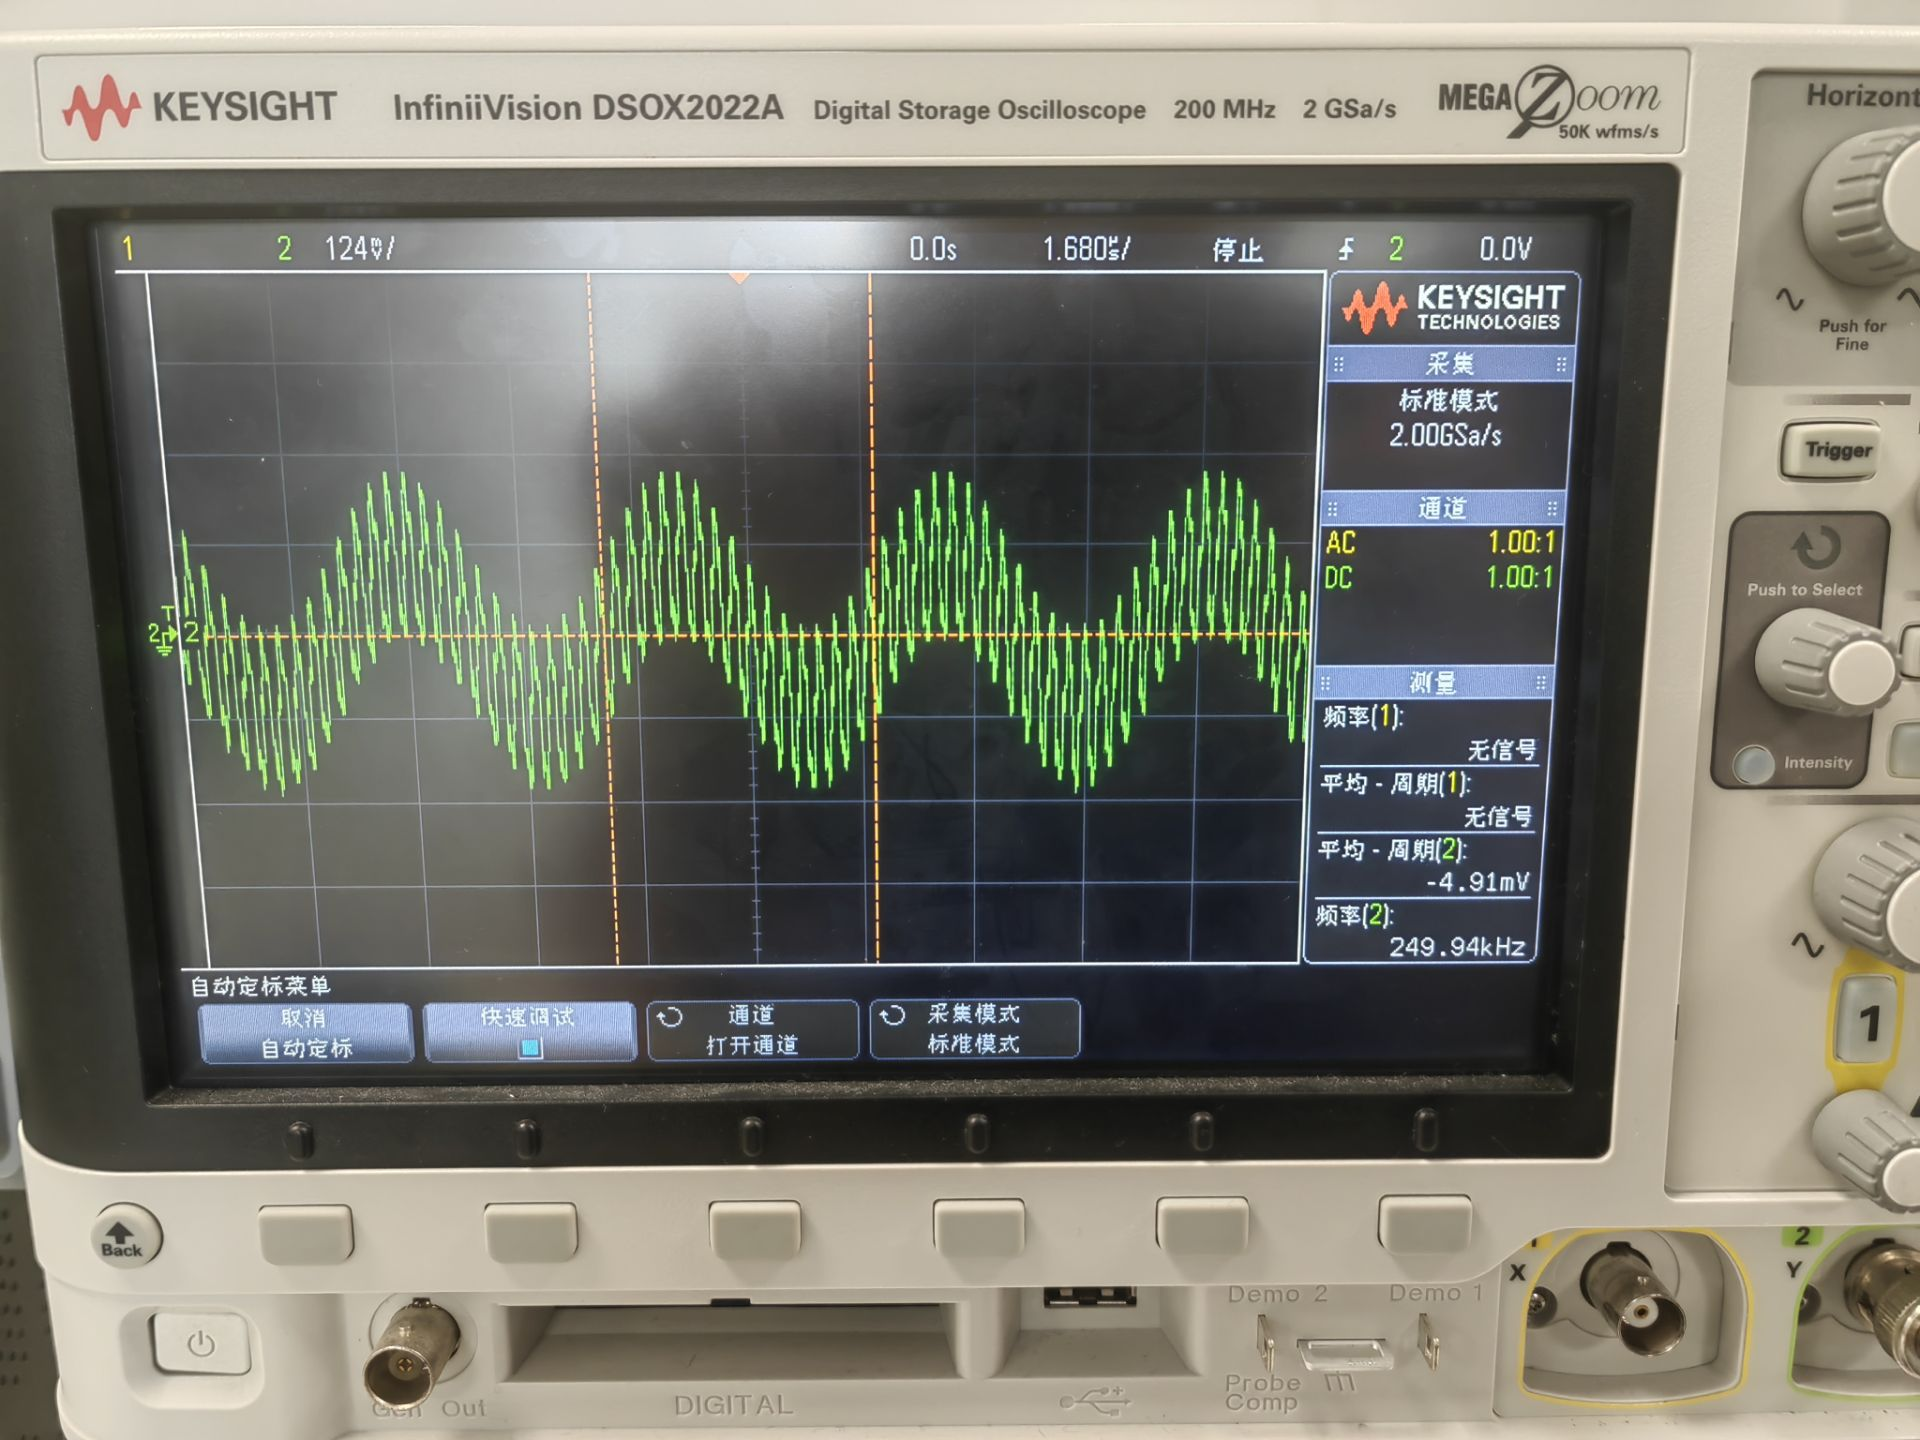
\includegraphics[width=0.35\textwidth]{figure/exp8/input.jpg}}
    \hspace{0.05\textwidth}
  \subfloat[输出信号]{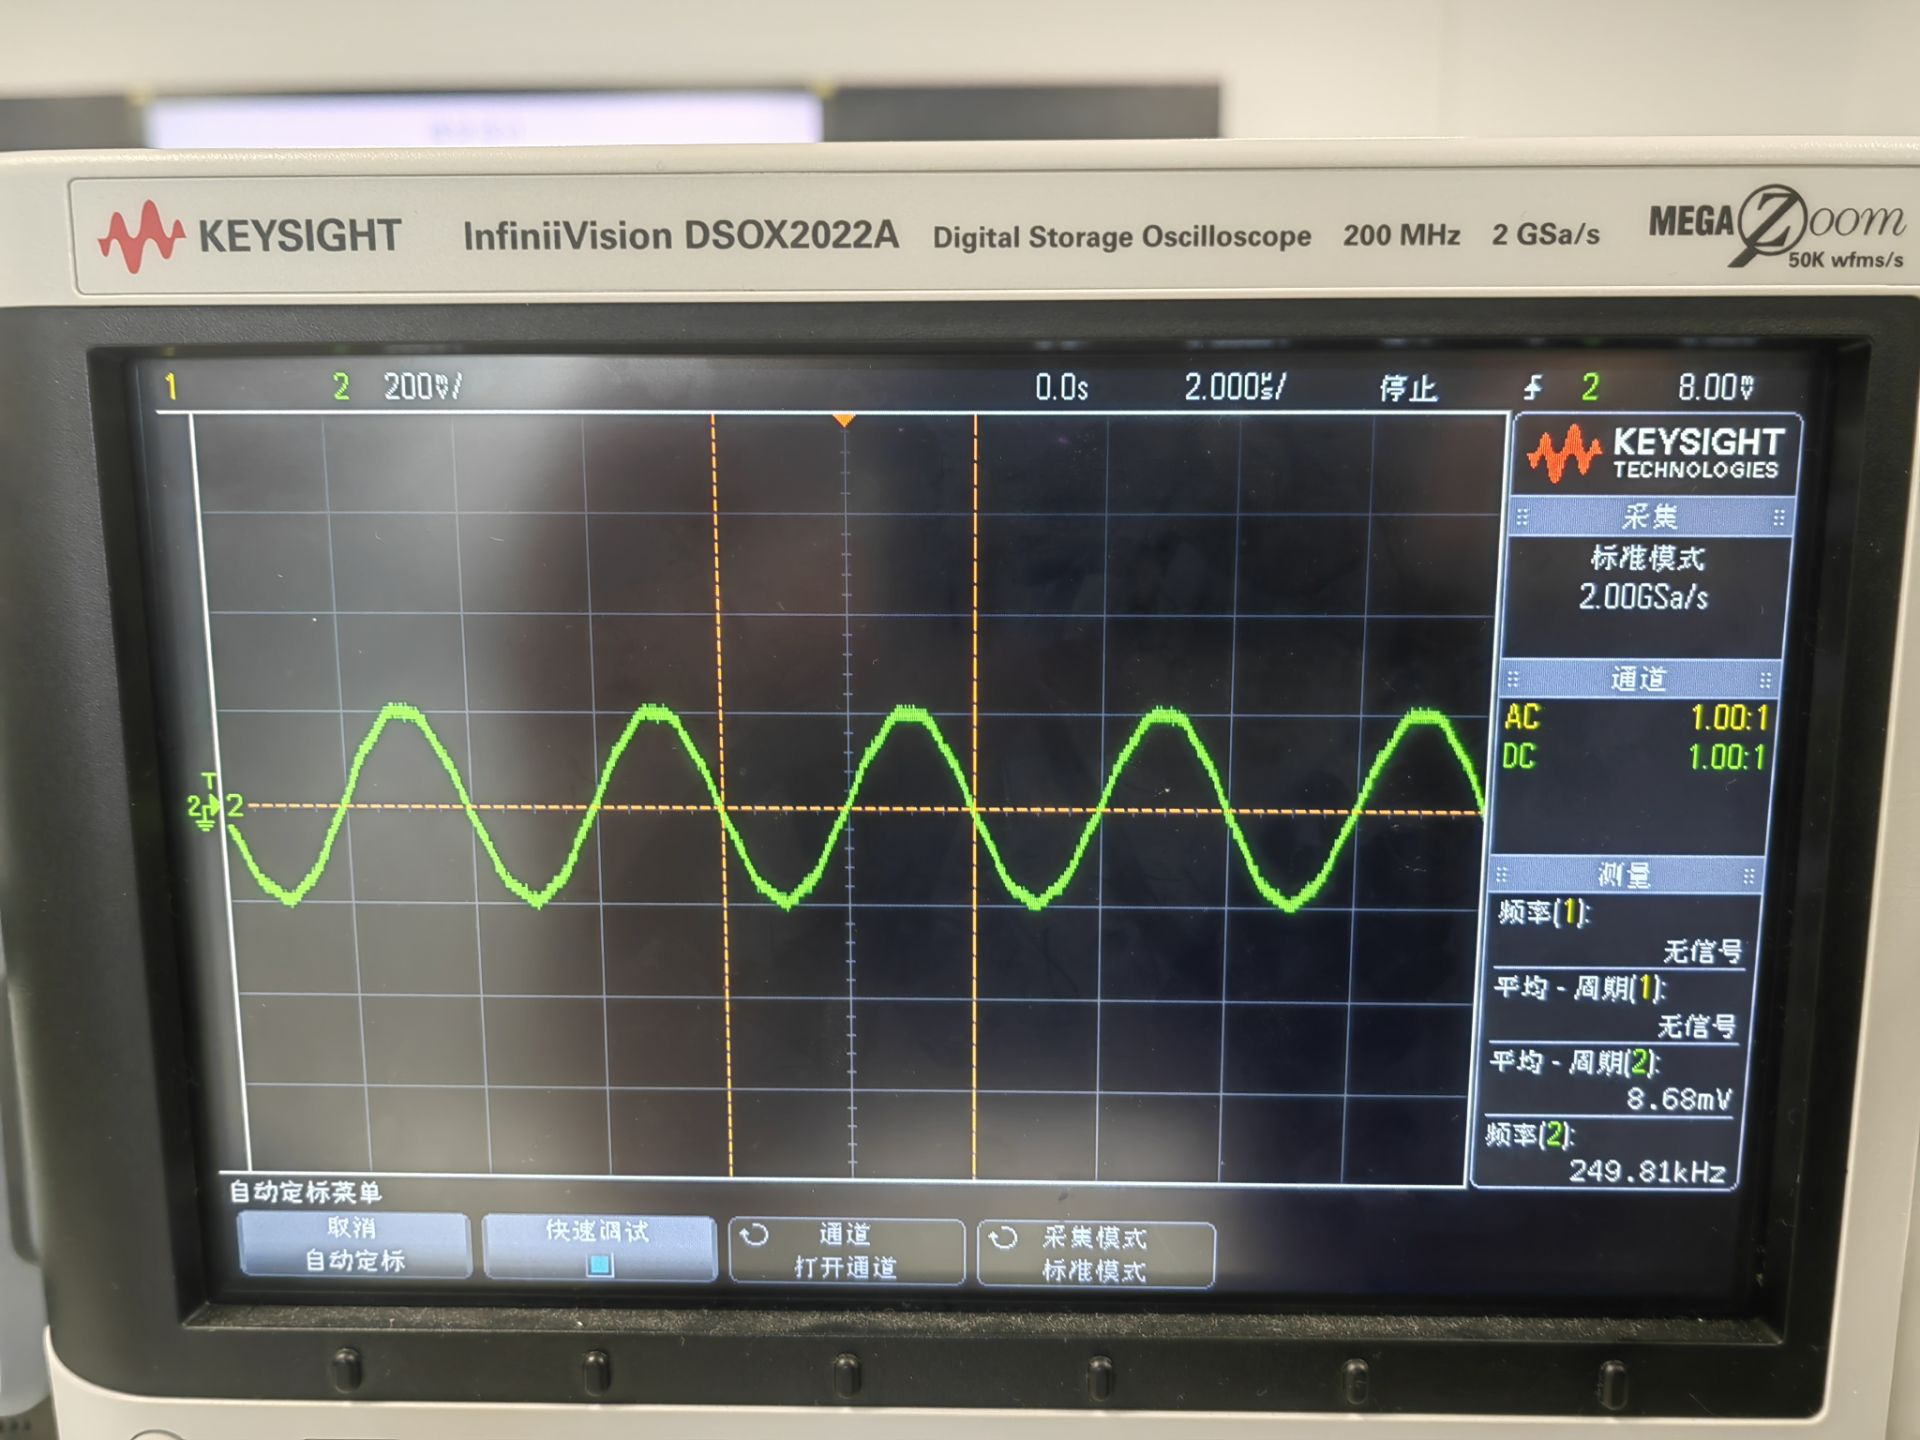
\includegraphics[width=0.35\textwidth]{figure/exp8/output.jpg}}
  \caption{IIR滤波器输入输出信号的示波器波形}
  \label{fig:exp8:waveform}
\end{figure}

打开硬件波形查看器ILA,可观察到输出波形中滤除了输入波形中的高频分量。(图~\ref{fig:exp8:sim:ILA})
\begin{figure}[htbp]
  \centering
  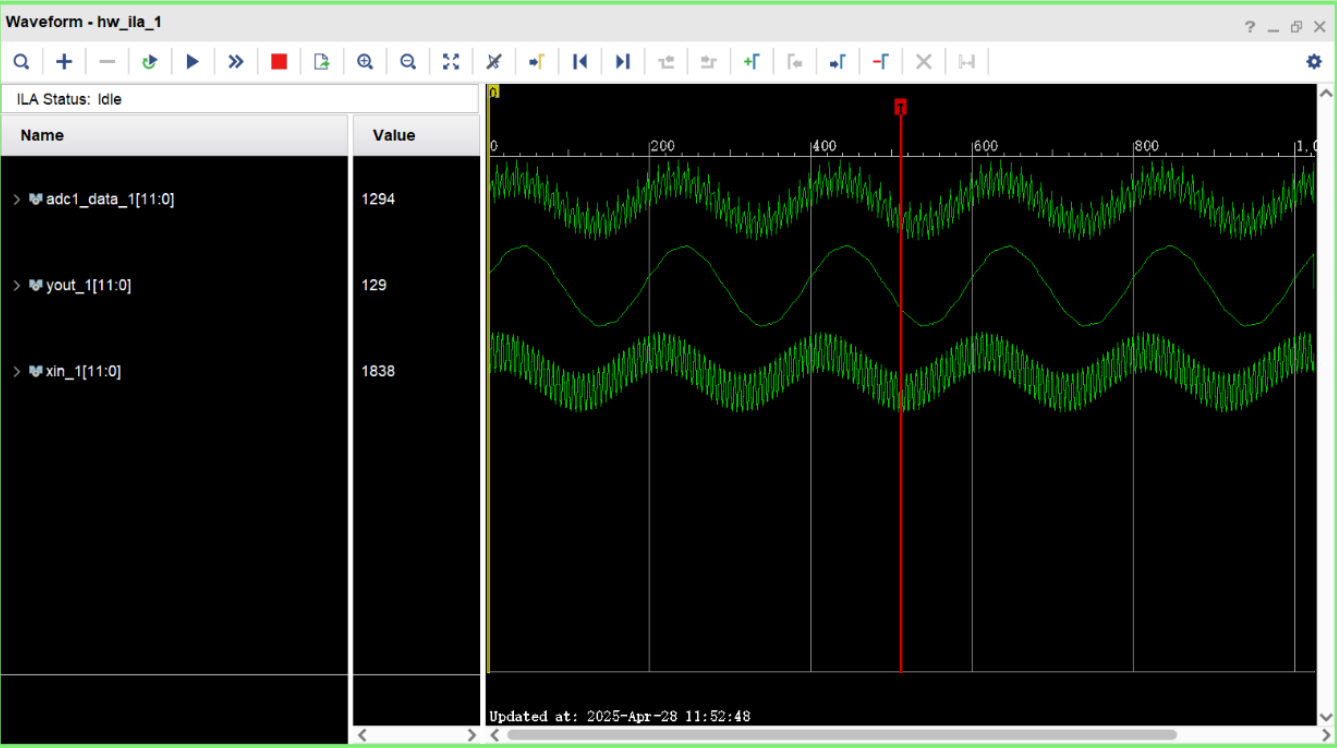
\includegraphics[width = 0.95\textwidth]{figure/exp8/ILA.png}
  \caption{ILA波形}
  \label{fig:exp8:sim:ILA}
\end{figure}

\subsection{资源消耗分析}
Vivado的资源报告如图~\ref{fig:exp8:resource_analysis}所示(包含TOP模块),展示了使用IIR滤波器在FPGA上的资源消耗情况。可以看到,设计使用了较少的LUT和FF资源,同时DSP资源的使用也在合理范围内。注意到FIR滤波器会使用MMCM资源,因此在实际使用时要合理分配FPGA资源。

\begin{figure}[htbp]
    \centering
    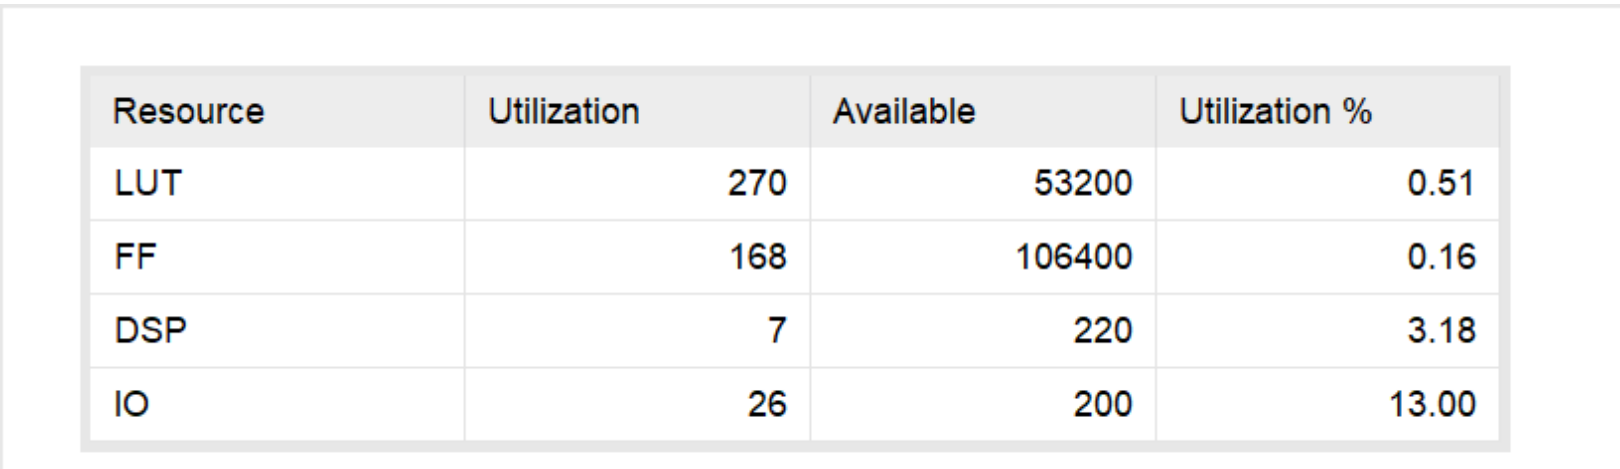
\includegraphics[width=0.45\textwidth]{figure/exp8/util_summary.png}
    \caption{资源消耗分析}
    \label{fig:exp8:resource_analysis}
\end{figure}
\subsection{时序分析}

时序分析表明,设计满足50MHz的时钟频率要求。
\begin{figure}[htbp]
    \centering
    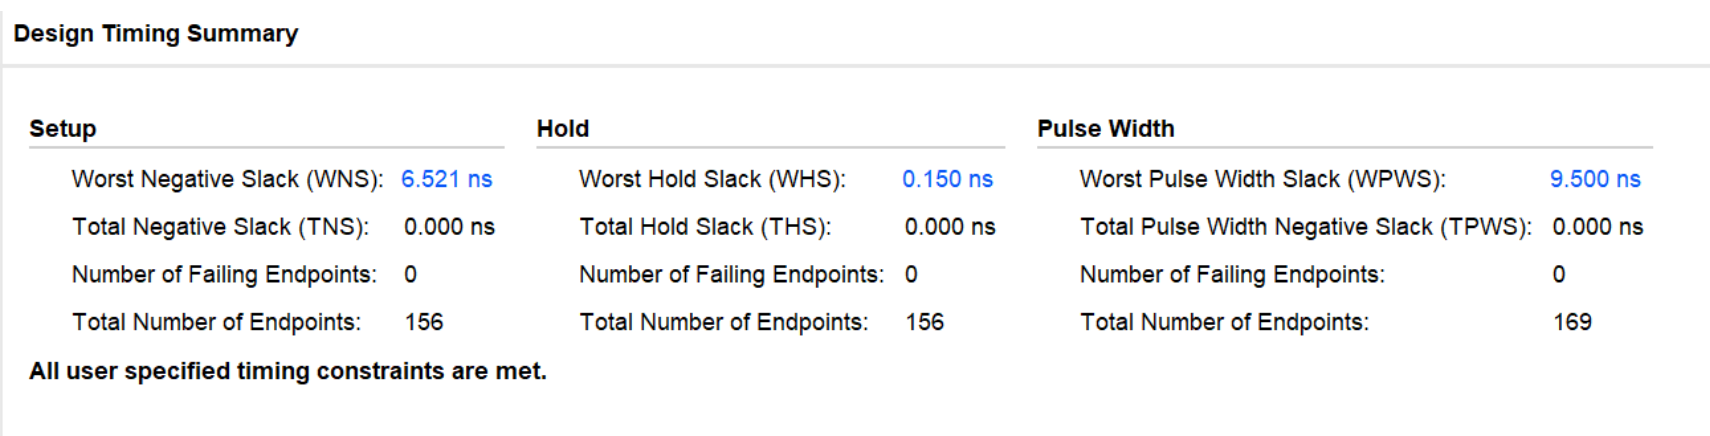
\includegraphics[width=0.8\textwidth]{figure/exp8/timing_summary.png}
    \caption{时序分析结果}
    \label{fig:exp8:time_analysis}
\end{figure}

具体分析:

\textbf{Setup:}  
\begin{itemize}
  \item Worst Negative Slack (WNS): 6.521 ns。表示最差的负时序余量,值为6.521纳秒,说明在时序上存在一定的余量,设计没有违反时序约束。  
\item Total Negative Slack (TNS): 0.00 ns。表示总的负时序余量为零,说明所有时序约束都被满足。  
\item Number of Failing Endpoints: 0。表示没有时序失败的端点,所有的时序约束都符合要求。  
\item Total Number of Endpoints: 156。表示在设计中,共有156个时序端点。
\end{itemize}


\textbf{Hold:}  
\begin{itemize}
\item Worst Hold Slack (WHS): 0.150 ns。表示最差的保持时序余量,值为0.150纳秒,表明该设计在保持时序方面没有违反约束。  
\item Total Hold Slack (THS): 0.00 ns。表示总的保持时序余量为零,表明所有保持时序约束都被满足。  
\item Number of Failing Endpoints: 0。表示没有违反保持时序约束的端点。  
\item Total Number of Endpoints: 5348。表示共有5348个端点。
\end{itemize}

\textbf{Pulse Width:}  
\begin{itemize}
  \item Worst Pulse Width Slack (WPWS): 9.000 ns。表示最差的脉冲宽度时序余量,值为9.000纳秒,说明设计在脉冲宽度方面有足够的时序余量。  
  \item Total Pulse Width Negative Slack (TPWS): 0.00 ns。表示总的脉冲宽度负时序余量为零,表明所有脉冲宽度时序约束都得到满足。  
  \item Number of Failing Endpoints: 0。表示没有违反脉冲宽度时序约束的端点。  
\item Total Number of Endpoints: 169。表示共有169个端点。
\end{itemize}

\section{思考与讨论}
\subsection{使用乘法器IP代替移位实现分子乘法}
代码如下:
\begin{lstlisting}[language=verilog,caption={使用乘法器IP代替移位实现分子乘法}]
module ZeroParallel (
    input rst, // Reset signal, active high
    input clk, // FPGA system clock, 50MHz
    input signed [11:0] Xin, // Input data, 50MHz
    output signed [20:0] Xout // Output filtered data
);
// Shift register for input samples
reg signed [11:0] Xin_Reg [6:0];
reg [3:0] i, j;
always @(posedge clk or posedge rst) begin
    if (rst) begin
        for (i = 0; i < 7; i = i + 1)
            Xin_Reg[i] <= 12'd0;
    end else begin
        for (j = 0; j < 6; j = j + 1)
            Xin_Reg[j+1] <= Xin_Reg[j];
    Xin_Reg[0] <= Xin;
    end
end
 // Sum symmetric inputs
wire signed [12:0] Add_Reg [3:0];
assign Add_Reg[0] = Xin + Xin_Reg[6];
assign Add_Reg[1] = Xin_Reg[0] + Xin_Reg[5];
assign Add_Reg[2] = Xin_Reg[1] + Xin_Reg[4];
assign Add_Reg[3] = Xin_Reg[2] + Xin_Reg[3];
// Coefficients for multipliers
wire signed [11:0] coe_zero [3:0];
assign coe_zero[0] = 12'd7; // *7
assign coe_zero[1] = 12'd21; // *21
assign coe_zero[2] = 12'd42; // *42
assign coe_zero[3] = 12'd56; // *56
// Multiplier outputs
wire signed [23:0] Mult_Reg [3:0]; 
MULT U_mult0 (.A (coe_zero[0]), .B (Add_Reg[0]), .P (Mult_Reg[0]));
MULT U_mult1 (.A (coe_zero[1]), .B (Add_Reg[1]), .P (Mult_Reg[1]));
MULT U_mult2 (.A (coe_zero[2]), .B (Add_Reg[2]), .P (Mult_Reg[2]));
MULT U_mult3 (.A (coe_zero[3]), .B (Add_Reg[3]), .P (Mult_Reg[3]));
// Sum the multiplication results
assign Xout = Mult_Reg[0][23:3] + Mult_Reg[1][23:3] + Mult_Reg[2][23:3] +
Mult_Reg[3][23:3];

endmodule
\end{lstlisting}
仿真结果:
\begin{figure}[htbp]
    \centering
    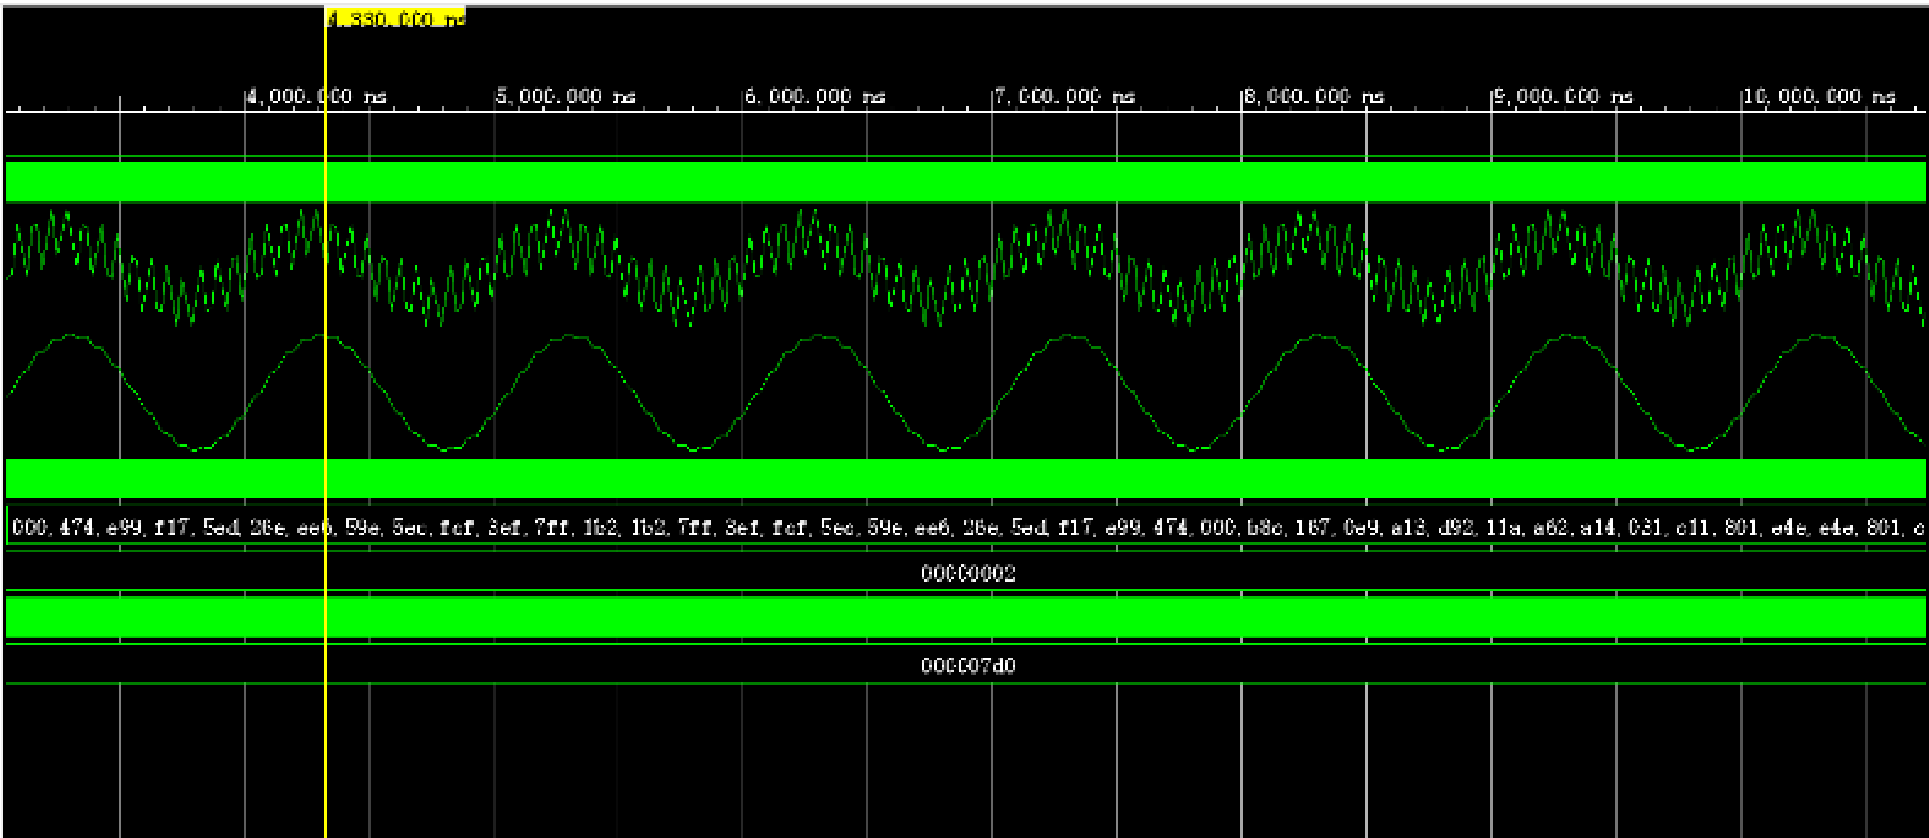
\includegraphics[width=0.8\textwidth]{figure/exp8/add-on.png}
    \caption{使用乘法器IP代替移位实现分子乘法的仿真结果}
    \label{fig:exp8:mult_ip_sim}
\end{figure}
这种方法使用了更多DSP,相对地减少了LUT的使用。

\subsection{IIR滤波器参数化设计}
利用下文中提到的实验流程加速框架,可以对IIR滤波器进行参数化设计。代码如下,可见用户只需要在python层传入\texttt{dwt\_din},\texttt{dwt\_dout},以及滤波器系数等参数就可以设计出正确位宽的IIR滤波器。IIR滤波器的内部参数通过python层的溢出逻辑判断,主要基于:
\begin{itemize}
    \item 乘法结果为输入位宽加和+1;
    \item 加法结果需要为输入位宽最大值+1
\end{itemize}
两条规则计算。

\begin{lstlisting}[language=python,caption = {IIR滤波器的参数化设计}]
from pytv.ModuleLoader import moduleloader
from pytv.Converter import convert
import math
import warnings

#NOTE This design is for max precision. May be different from the one in the guideline.
@convert
def Moduleiir_direct(din_name = "din", dout_name = "dout", dwt_din: int = 12, dwt_dout: int = 12, if_rst_n = True, num_coeffs = [7,21,42,56], denom_coeffs = [-922, 1163, -811, 412, -122, 24, -2], zero_IP = True,zero_MULT_IP = "MULT", pole_MULT_IP = "MULT"):
    # Reserve enough bits for num/denom outputs
    # The adder overflow is considered.
    zero_output_maxbits = dwt_din + 1 + max(len(bin(abs(coeff))) - 2 for coeff in num_coeffs) + math.ceil(math.log2(len(num_coeffs))) # +1 for the addition, -2 for the '0b'
    
    pole_output_maxbits = dwt_dout + 1 + max(len(bin(abs(coeff))) - 2 for coeff in denom_coeffs) + math.ceil(math.log2(len(denom_coeffs))) # +1 for the addition
    
    #/`timescale 1ns / 1ps
    #/ module IIRDirect (
    #/     input rst,               // Reset signal, active high
    #/     input clk,               // FPGA system clock, 50MHz
    #/     input signed [`dwt_din-1`:0] `din_name`,  // Input data
    #/     output signed [`dwt_dout-1`:0] `dout_name` // Output filtered data
    #/ );
    #/ 
    #/     // Instantiate Zero Parallel block
    #/     wire signed [`zero_output_maxbits-1`:0] Xout;
    inst_zero_parallel = {"rst": "rst", "clk": "clk", "Xin": "din", "Xout": "Xout"}
    if zero_IP:
        Modulezero_parallel(MULT_IP_NAME=zero_MULT_IP, dwt_xin= dwt_din, dwt_yout= zero_output_maxbits, if_rst_n=True, zero_coeffs= num_coeffs, PORTS = inst_zero_parallel)
    else:
        Modulezero_parallel_shift(dwt_xin= dwt_din, dwt_yout= zero_output_maxbits, if_rst_n=True, zero_coeffs= num_coeffs, PORTS = inst_zero_parallel)
    #/ 
    #/     // Instantiate Pole Parallel block
    #/     wire signed [`dwt_dout-1`:0] Yin;
    #/     wire signed [`pole_output_maxbits-1`:0] Yout;
    inst_pole_parallel = {"rst": "rst", "clk": "clk", "Yin": "Yin", "Yout": "Yout"}
    Modulepole_parallel(MULT_IP_NAME=pole_MULT_IP, dwt_yin= dwt_dout, dwt_yout= pole_output_maxbits, if_rst_n=True, pole_coeffs= denom_coeffs, PORTS = inst_pole_parallel)
    #/ 
    #/     // Calculate output: (Zero - Pole) / 512
    #/     wire signed [`pole_output_maxbits-1`:0] Ysum;
    #/
    pad_size = pole_output_maxbits - zero_output_maxbits
    #/     assign Ysum = {{`pad_size`{Xout[`zero_output_maxbits`-1]}}, Xout} - Yout;
    #/ 
    #/     wire signed [`pole_output_maxbits-1`:0] Ydiv;
    #/ 
    arithmetic_shift = zero_output_maxbits - dwt_dout
    if arithmetic_shift > 0:
        #/     assign Ydiv = {{`arithmetic_shift`{Ysum[`pole_output_maxbits-1`]}}, Ysum[`pole_output_maxbits-1`:`arithmetic_shift`]}; // Arithmetic shift the numerator result `arithmetic_shift` bits to fit denominator's input size
        pass
    else:
        #/     assign Ydiv = Ysum;
        pass
    #/ 
    #/     // Final output assignment
    #/     assign Yin  = (!rst ? `dwt_dout`'d0 : Ydiv[`dwt_dout-1`:0]);
    #/     assign `dout_name` = Yin;
    #/ 
    #/ endmodule


    pass
    

@convert
def Modulezero_parallel_shift(xin="Xin", yout="Xout", dwt_xin: int = 12, dwt_yout: int = 26, zero_coeffs=None, if_rst_n=True):
    """
    Parameters:
    - xin: Input signal name
    - yout: Output signal name
    - dwt_xin: Input bit width
    - dwt_yout: Output bit width
    - zero_coeffs: List of zero coefficients (e.g., [7, 21, 42, 56])
    - if_rst_n: Whether to include reset signal
    """
    if zero_coeffs is None:
        zero_coeffs = [7, 21, 42, 56]  # Default coefficients
        
    # Check for potential overflow
    max_result_bits = dwt_xin + 1 + max(len(bin(coeff)[2:]) for coeff in zero_coeffs)  # +1 for the addition
    if max_result_bits > dwt_yout:
        warnings.warn(f"The module may produce overflow results: "
                     f"dwt_xin={dwt_xin} bits + coefficients (max {max(zero_coeffs)}) "
                     f"require {max_result_bits} bits, but dwt_yout is only {dwt_yout} bits.")
                     
    num_coeffs = len(zero_coeffs)
    # Calculate required internal bit width to prevent overflow
    # The multiplier output width should account for coefficient accumulation
    # We need extra bits to accommodate sum of all coefficients (log2 of the number of terms)
    internal_bit_width = dwt_yout - math.floor(math.log2(num_coeffs))
    #/ module ZERO_PARALLEL (
    #/ 
    if if_rst_n:
        #/  rst,
        pass
    #/  clk, `xin`, `yout`
    #/ );
    #/ 
    #/ input clk;
    if if_rst_n:
        #/ input rst;
        pass
    #/ input signed [`dwt_xin-1`:0] `xin`;
    #/ output signed [`dwt_yout-1`:0] `yout`;
    #/ 
    #/ // Shift register for input samples
    #/ reg signed [`dwt_xin-1`:0] Xin_Reg [`num_coeffs-1`:0];
    
    #/ always @(posedge clk or negedge rst) begin
    #/      if (!rst) begin
    for i in range(num_coeffs):
        #/          Xin_Reg[`i`] <= `dwt_xin`'d0;
        pass
    #/      end else begin
    for j in range(num_coeffs - 1):
        #/          Xin_Reg[`j+1`] <= Xin_Reg[`j`];
        pass
    #/          end 
    #/          Xin_Reg[0] <= `xin`;
    #/      end
    #/ end
    #/ 
    #/ // Sum symmetric inputs
    #/ wire signed [`dwt_xin`:0] Add_Reg [`num_coeffs/2-1`:0];
    for i in range(num_coeffs // 2):
        #/ assign Add_Reg[`i`] = Xin_Reg[`i`] + Xin_Reg[`num_coeffs-1-i`];
        pass
    #/ 
    #/ // Multiply by coefficients using shifts and additions
    #/ wire signed [`internal_bit_width-1`:0] Mult_Reg [`num_coeffs/2-1`:0];
    for i, coeff in enumerate(zero_coeffs[:num_coeffs // 2]):
        shifts = []
        for shift, bit in enumerate(bin(coeff)[2:][::-1]):  # Reverse binary representation
            if bit == '1':
                shifts.append(f"{{{shift+ dwt_xin}}}, Add_Reg[{i}], {shift}'d0")
        shift_expr = " + ".join(shifts)
        #/ assign Mult_Reg[`i`] = `shift_expr`; // *coeff
        pass
    #/ 
    #/ // Sum results
    output_str = f"Mult_Reg[0]"
    for i in range(1, num_coeffs // 2):
        output_str = output_str + f"Mult_Reg[{i}]"
        pass
    #/ assign `yout` = `output_str`;
    #/ endmodule
    pass

@convert
def Modulezero_parallel(xin="Xin", yout="Xout", dwt_xin: int = 12, dwt_yout: int = 26, zero_coeffs=None, MULT_IP_NAME="MULT", if_rst_n=True):
    """
    Parameters:
    - xin: Input signal name
    - yout: Output signal name
    - dwt_xin: Input bit width
    - dwt_yout: Output bit width
    - zero_coeffs: List of zero coefficients (e.g., [7, 21, 42, 56])
    - MULT_IP_NAME: Name of the multiplier IP
    - if_rst_n: Whether to include reset signal
    """
    if zero_coeffs is None:
        zero_coeffs = [7, 21, 42, 56]  # Default coefficients

    num_coeffs = len(zero_coeffs)
    # Calculate required internal bit width to prevent overflow
    # The multiplier output width should account for coefficient accumulation
    # We need extra bits to accommodate sum of all coefficients (log2 of the number of terms)
    internal_bit_width = dwt_yout - math.floor(math.log2(num_coeffs))
    print(f"Note: The {MULT_IP_NAME} IP must have an output width of at least {internal_bit_width} bits to prevent adder overflow")
    #/ module ZERO_PARALLEL (
    #/ 
    if if_rst_n:
        #/  rst,
        pass
    #/  clk, `xin`, `yout`
    #/ );
    #/ 
    #/ input clk;
    if if_rst_n:
        #/ input rst;
        pass
    #/ input signed [`dwt_xin-1`:0] `xin`;
    #/ output signed [`dwt_yout-1`:0] `yout`;
    #/ 
    #/ // Shift register for input samples
    #/ reg signed [`dwt_xin-1`:0] Xin_Reg [`num_coeffs-1`:0];
    #/ always @(posedge clk or negedge rst) begin
    #/      if (!rst) begin
    for i in range(num_coeffs):
        #/ Xin_Reg[`i`] <= `dwt_xin`'d0;
        pass
    #/      end else begin
    for j in range(num_coeffs - 1):
        #/ Xin_Reg[`j+1`] <= Xin_Reg[`j`];
        pass
    #/          end 
    #/          Xin_Reg[0] <= `xin`;
    #/      end
    #/ end
    #/ 
    #/ // Sum symmetric inputs
    #/ wire signed [`dwt_xin`:0] Add_Reg [`num_coeffs/2-1`:0];
    for i in range(num_coeffs // 2):
        #/ assign Add_Reg[`i`] = Xin_Reg[`i`] + Xin_Reg[`num_coeffs-1-i`];
        pass
    #/ 
    #/ // Multiply by coefficients using IP cores
    #/ wire signed [`internal_bit_width-1`:0] Mult_Reg [`num_coeffs/2-1`:0];
    for i, coeff in enumerate(zero_coeffs[:num_coeffs // 2]):
        #/ `MULT_IP_NAME` Umult`i` (.A(Add_Reg[`i`]), .B(`dwt_xin`'d`coeff`), .P(Mult_Reg[`i`]));
        pass
    #/ 
    #/ // Sum results
    output_str = f"Mult_Reg[0]"
    for i in range(1, num_coeffs // 2):
        output_str += f" + Mult_Reg[{i}]"
    #/ assign `yout` = `output_str`;
    #/ endmodule
    pass


@convert
def Modulepole_parallel(yin="Yin", yout="Yout", dwt_yin: int = 12, dwt_yout: int = 26, pole_coeffs=None, MULT_IP_NAME="MULT", if_rst_n=True):
    """
    Parameters:
        yin: Input signal name
        yout: Output signal name
        dwt_yin: Input bit width
        dwt_yout: Output bit width
        pole_coeffs: List of pole coefficients (e.g., [-922, 1163, -811, 412, -122, 24, -2])
        MULT_IP_NAME: Name of the multiplier IP
        if_rst_n: Whether to include reset signal
    """
    if pole_coeffs is None:
        pole_coeffs = [-922, 1163, -811, 412, -122, 24, -2]  # Default coefficients (Decimal)

    num_coeffs = len(pole_coeffs)
    coe_width = max(len(bin(abs(coeff))) - 2 for coeff in pole_coeffs)  # +1 for the sign
    # Calculate required internal bit width to prevent overflow
    # The multiplier output width should account for coefficient accumulation
    # We need extra bits to accommodate sum of all coefficients (log2 of the number of terms)
    internal_bit_width = dwt_yout - math.floor(math.log2(num_coeffs))
    print(f"Note: The {MULT_IP_NAME} IP must have an output width of at least {internal_bit_width} bits to prevent adder overflow")
    
    #/`timescale 1ns / 1ps
    #/ module POLE_PARALLEL (
    #/ 
    if if_rst_n:
        #/  rst,
        pass
    #/  clk, `yin`, `yout`
    #/ );
    #/ 
    #/ input clk;
    if if_rst_n:
        #/ input rst;
        pass
    #/ input signed [`dwt_yin-1`:0] `yin`;
    #/ output signed [`dwt_yout-1`:0] `yout`;
    #/ 
    #/ // Shift register for previous outputs
    #/ reg signed [`dwt_yin-1`:0] Yin_Reg [`num_coeffs-1`:0];
    #/ reg [3:0] i, j;
    #/ always @(posedge clk or negedge rst) begin
    #/     if (!rst) begin
    for i in range(num_coeffs):
        #/         Yin_Reg[`i`] <= `dwt_yin`'d0;
        pass
    #/     end else begin
    for j in range(num_coeffs - 1):
        #/         Yin_Reg[`j+1`] <= Yin_Reg[`j`];
        pass
    #/         Yin_Reg[0] <= `yin`;
    #/     end
    #/ end
    #/ 
    #/ // Coefficients (user-defined)
    #/ wire signed [`coe_width-1`:0] coe [`num_coeffs-1`:0];
    for i, coeff in enumerate(pole_coeffs):
        #/ assign coe[`i`] = `coeff`;
        pass
    #/ 
    #/ // Multiplier outputs
    #/ wire signed [`internal_bit_width-1`:0] Mult_Reg [`num_coeffs-1`:0];
    for i in range(num_coeffs):
        #/ `MULT_IP_NAME` Umult`i` (.A(coe[`i`]), .B(Yin_Reg[`i`]), .P(Mult_Reg[`i`]));
        pass
    #/ 
    #/ // Sum multiplier outputs
    output_str = f"Mult_Reg[0]"
    for i in range(1, num_coeffs):
        output_str += f" + Mult_Reg[{i}]"
    #/ assign `yout` = `output_str`;
    #/ endmodule
    pass
\end{lstlisting}

\subsection{实验流程加速框架简述}
在《系统实验》这门课这次以及之前的实验中,可以发现一次完整的信号分析流程大抵相同,主要包括以下几个步骤:
\begin{itemize}
    \item 通过FFT IP核的功能仿真确定待滤波信号频谱(实验需求);
    \item 指定滤波器类型,输入信号频率,采样频率等;
    \item 使用高级语言,如MATLAB的\texttt{Filter Designer}工具生成滤波器系数,验证幅频响应,并导出COE系数文件用作滤波器系数;
    \item 编写RTL代码或调用IP核,实现滤波器的硬件设计;
    \item 编写测试Testbench,进行功能仿真验证,并验证时序是否违例,生成资源消耗情况报告;
    \item 使用ADC或DDS输入数据,例化相应IP核,并设置ILA观测信号接口。
    \item 写比特流验证,通过配套硬件接口,如eNodeX 30B软件无线电创新平台进行硬件验证。在此过程中通过ILA观察输入输出信号的波形。
\end{itemize}

传统的实验方式需要每次从MATLAB GUI中手动导出COE文件,并在Vivado FIR IP核中引用该COE文件。并且,现有的设计流程需要每次在RTL设计中修改输入输出位宽,并手动修改FIR和FFT IP核的配置参数,过程繁杂且易出错,无法满足快速参数化设计的需求。为此,我们提出一种基于python \texttt{matplotlib, scipy, verithon} 库和Vivado tcl脚本的设计流程加速框架。目前,用户可以基于此框架完成以下功能:
\begin{itemize}
    \item 生成任意幅度、相位、长度的正弦序列,并支持信号运算、信号定点量化、信号时域/频域分析和信号导出(COE格式或TXT格式);
    \item 使用\texttt{scipy.signal}库设计FIR、IIR滤波器(滤波效果劣于filterDesigner,但自动化程度更高),用户仅需传入滤波器类型、采样频率、通带阻带边界、滤波器阶数、量化位宽参数,即可自动生成滤波器系数和查看滤波器幅频响应,并提供导出COE格式文件的API;
    \item 提供FFT、串行、并行、半串行FIR滤波器、IIR滤波器的设计模板(基于做过的实验),用户在python层指定参数后,即可自动生成正确位宽的RTL代码。
    \item 提供\texttt{FIR compiler}, \texttt{xfft} IP核的tcl脚本,系统目前支持自动推断IP核需修改的配置参数。
    \item 提供自动生成Testbench的API(文件读写形式的测试),用户可以灵活地指定时钟、复位和输入输出形式。
\end{itemize}

目前该框架还在不断完善中,由于即将期末考试,对该项目的开发有所延缓。后续会继续完善该框架,力求实现自动化的实验流程。项目代码目前托管在Github上,地址为\url{https://github.com/LiPtP0000/system_experiment_autogen}。